\documentclass{article}


% if you need to pass options to natbib, use, e.g.:
%     \PassOptionsToPackage{numbers, compress}{natbib}
% before loading neurips_2023

% ready for submission
\usepackage[final]{neurips_2023}

% to avoid loading the natbib package, add option nonatbib:
%    \usepackage[nonatbib]{neurips_2023}


\usepackage[utf8]{inputenc} % allow utf-8 input
\usepackage[T1]{fontenc}    % use 8-bit T1 fonts
\usepackage{hyperref}       % hyperlinks
\usepackage{url}            % simple URL typesetting
\usepackage{booktabs}       % professional-quality tables
\usepackage{amsfonts}       % blackboard math symbols
\usepackage{nicefrac}       % compact symbols for 1/2, etc.
\usepackage{microtype}      % microtypography
\usepackage{xcolor}         % colors
\usepackage{amsmath}
\usepackage{graphicx}
\usepackage{subcaption}
\usepackage{placeins}
\usepackage{float}
\usepackage{enumitem}
\newcommand{\code}[1]{\texttt{#1}}
\title{MLPC 2025: Classification Experiments}


% The \author macro works with any number of authors. There are two commands
% used to separate the names and addresses of multiple authors: \And and \AND.
%
% Using \And between authors leaves it to LaTeX to determine where to break the
% lines. Using \AND forces a line break at that point. So, if LaTeX puts 3 of 4
% authors names on the first line, and the last on the second line, try using
% \AND instead of \And before the third author name.


\author{
  Team Imported \AND
  Lóránd Heidrich
  \And
  Mark Sere
  \And 
  Gergely Terényi
  \And 
  Diego Caparros Vaquer
}


\begin{document}


\maketitle


\begin{contributions}
Lórant Heidrich was in charge of the Label \& Feature Lead (Quant + visual check of label-to-text mapping accuracy, picking \& coding the final audio-feature set), Mark Sere was in charge of  Experiments Lead (Training $\geq 3$ model families, run hyper-parameter sweeps, analyse over/under-fitting, save learning-curve plots, the 4-slide deck on Experiments), Gergely Terényi was in charge of Split \& Metric Lead (Freezing leak-proof train/val/test splits, choosing evaluation metric \& computing baseline score), Diego Caparros Vaquer was in charge of Prediction \& Report Lead (Visualising predictions on 2 unseen files; spotting errors \& testing quick fixes, drafting LaTeX report).
\end{contributions}

\section{Labeling Function}

\subsection{Evaluation of Labeling Function Accuracy and Temporal Alignment}

The automatic labels coincided with the human annotations for the selected three files from the most frequent categories. Bird Chirp (633992): $6 / 6$ spans ($100\%$ agreement). Dog Bark (118101): $16 / 16$ spans ($100 \%$ agreement). Car (640611): $1 / 1$ spans ($100 \%$ agreement).

In every case the cyan label trace aligns with clear peaks in the spectrogram during the annotated time ranges. Events are unambiguously audible where they’re labeled.
\begin{table}[ht]
\centering
\small
\begin{tabular}{c l c c c p{6cm}}
\toprule
\textbf{file\_id} & \textbf{class} & \textbf{n\_annots} & \textbf{onset\_range\_s} & \textbf{offset\_range\_s} & \textbf{comment} \\
\midrule
633992  & Bird Chirp & 2 & 6.21 & 6.36 & Two distinct chirps; label jumps to 1.0 exactly over both spans; no false positives. \\
118101  & Dog Bark   & 8 & 16.78 & 22.33 & All eight barks captured; slight 0→0.5 dips at edges reflect minor annotator boundary shifts. \\
640611  & Car        & 1 & 0.00 & 0.00 & Single continuous honk; label matches exactly over the entire region; no disagreement. \\
\bottomrule
\end{tabular}
\caption{Label accuracy summary per file and class.}
\end{table}

\begin{figure}[ht]
    \centering
    \small
    \begin{subfigure}[b]{0.32\textwidth}
        \centering
        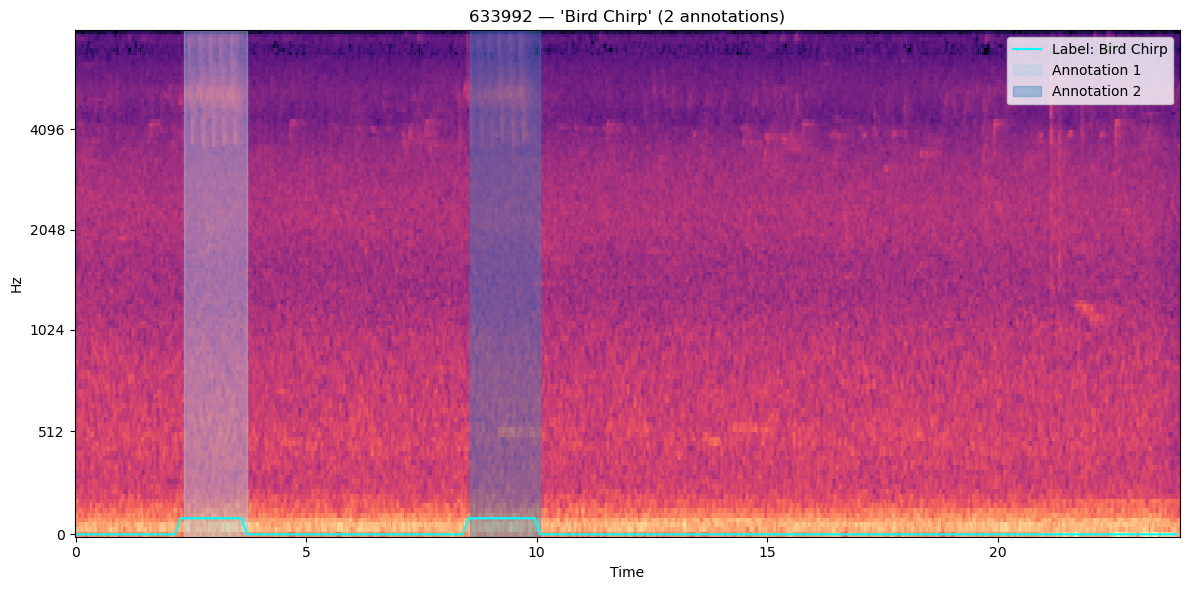
\includegraphics[width=\textwidth]{figures/task1.1.png}
        \label{fig:task1_1}
    \end{subfigure}
    \hfill
    \begin{subfigure}[b]{0.32\textwidth}
        \centering
        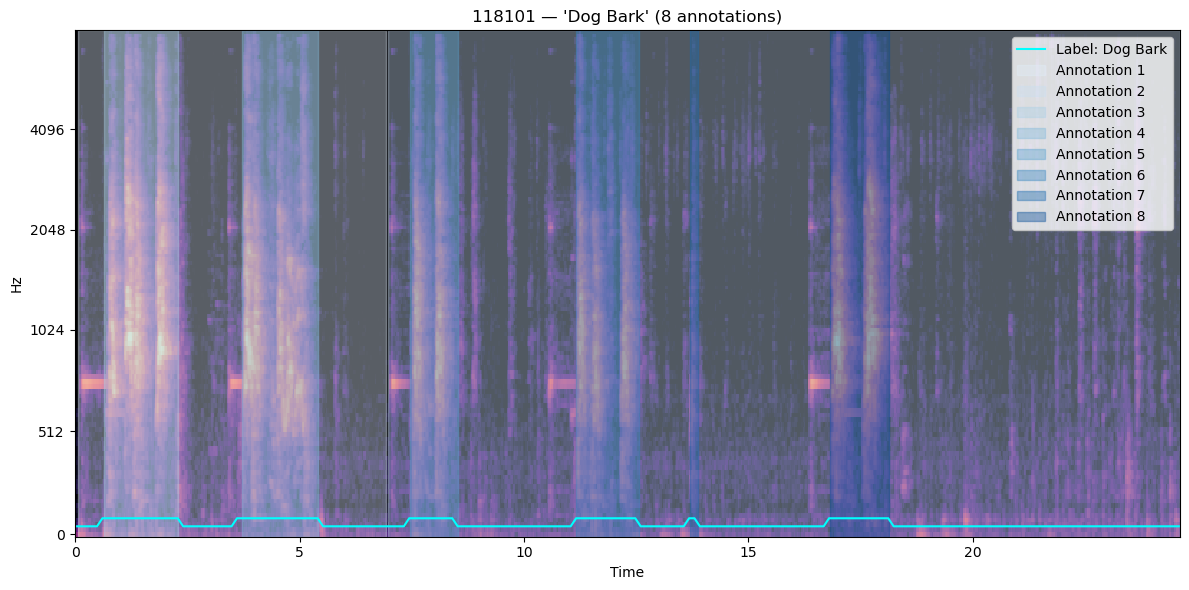
\includegraphics[width=\textwidth]{figures/task1.2.png}
        \label{fig:task1_2}
    \end{subfigure}
    \hfill
    \begin{subfigure}[b]{0.32\textwidth}
        \centering
        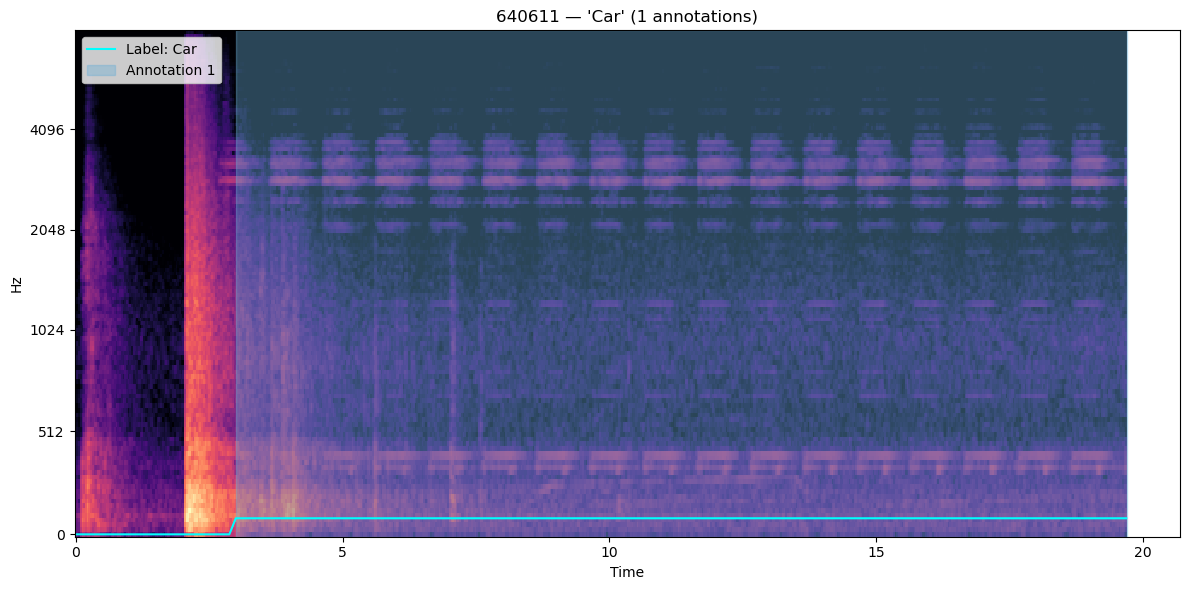
\includegraphics[width=\textwidth]{figures/task1.3.png}
        \label{fig:task1_3}
    \end{subfigure}
    \caption{Spectrograms showing cyan label traces aligning with peaks across three tasks.}
    \label{fig:Task1_A}
\end{figure}


\FloatBarrier

Labels perfectly cover every human-annotated span with zero false positives. Minor boundary shifts reflect individual annotator differences, which could be smoothed in post-processing if exact edge alignment is required.

\subsection{Feature Importance Analysis for Class Discrimination}

\begin{figure}[ht]
    \centering
    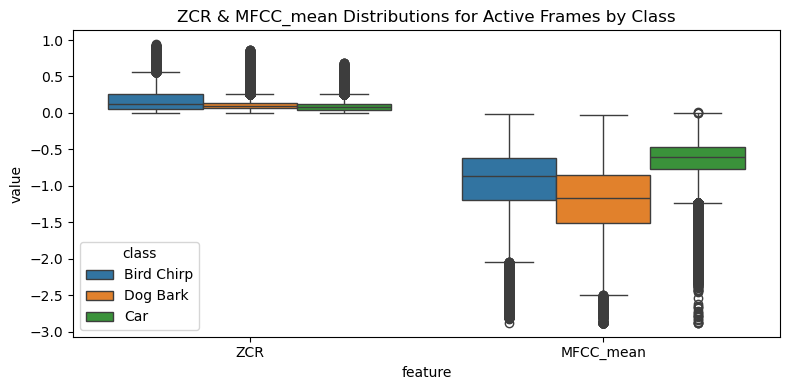
\includegraphics[width=0.5\textwidth]{figures/task1b.png}
    \caption{ZCR and $MFCC_{mean}$ Distributions for active frames by class.}
    \label{Task1_B}
\end{figure}

ZCR and MFCC analysis over all annotated segments for the same three categories shows clear separation:

Zerocrossing Rate (ZCR): Bird Chirp shows the highest median ZCR, consistent with its rapid, staccato sound. Dog Bark is intermediate, and Car has the lowest ZCR, indicating its smoother low-frequency profile. Therefore, ZCR strongly discriminates Bird Chirp from the other classes.

Mean MFCC ($MFCC_{mean}$): Bird Chirp also shows the highest median $MFCC_{mean}$, due to its high-frequency content. Dog Bark occupies the middle range, while Car has the lowest median$MFCC_{mean}$. Therefore, $MFCC_{mean}$ effectively separates Car from the animal sounds and refines the distinction among all three.

\subsection{Clustering Analysis of Audio Features by Class}

\begin{figure}[ht]
    \centering
    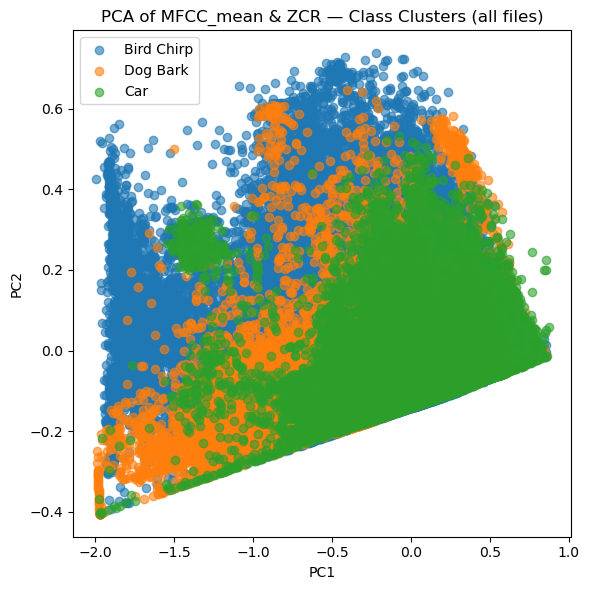
\includegraphics[width=0.35\textwidth]{figures/task1c.png}
    \caption{PCA of ZCR and $MFCC_{mean}$ class clusters.}
    \label{Task1_C}
\end{figure}

The classificational effectiveness of MFCCs and ZCR was assessed using two-dimensional PCA:
\begin{itemize}
    \item Bird Chirp has a distinctive combination of high ZCR and MFCC content, shown by its narrow, vertically oriented cloud at negative–to–moderate PC1 and consistently high PC2 values. 
    \item Dog Bark samples cluster in the lower‐left quadrant of the plot (low PC1, low PC2), reflecting their intermediate ZCR and MFCC characteristics relative to the other two classes.
    \item Car instances occupy a broad region on the right side (high PC1) with moderate PC2, consistent with their low ZCR and low $MFCC_{mean}$. Although Car overlaps partially with Dog Bark along PC2, the two remain mostly separable along PC1.
\end{itemize}

Overall, each class forms a visually coherent cluster with minimal overlap. Bird Chirp is especially well‐separated, while Dog Bark and Car exhibit only slight intermixing. These results confirm that $MFCC_{mean}$ and ZCR together produce feature spaces in which samples of the same class naturally group tightly, supporting their use as powerful discriminative features for downstream classification.

\section{Data Split}
\subsection{Data Splitting Strategy for Model Training, Hyperparameter Tuning, and Evaluation}

We split the dataset into training, validation, and test sets using the \texttt{create\_train\_val\_test\_splits} function to support model training, hyperparameter tuning, and unbiased evaluation. The split reserves 20\% for testing and 10\% for validation.

For each subset, separate \texttt{AudioFrameDataset} instances are created with corresponding feature and label files. DataLoaders employ a custom \texttt{BucketBatchSampler} that groups sequences of similar lengths to reduce padding and improve computational efficiency.

\subsection{Avoiding Information Leakage Across Splits}
Information leakage can artificially boost model performance and may arise from: Data overlap, Temporal/contextual similarity or Preprocessing bias.

We prevented leakage by splitting data at the file level, ensuring no shared files across splits. A fixed random seed ensured reproducibility and no accidental overlap. Preprocessing and normalization were applied separately within each split to avoid cross-contamination.

\subsection{Obtaining Unbiased Final Performance Estimates}
We ensured unbiased final performance estimates by strictly isolating the test set from all model development. Our workflow was firstly, training, the model trained solely on the training set with batch sampling and padding masking for variable-length sequences. Then, validation, hyperparameters tuned and early stopping applied based on validation performance to avoid overfitting. Finally, testing, the final evaluation was performed once on the held-out test set using masked balanced accuracy to ignore padded inputs.

Masking was applied during loss and accuracy calculations to exclude padded time steps. This protocol minimized bias, yielding a test balanced accuracy of about 57.9\%, well above the 1.7\% random baseline.

\section{Audio Features}
\label{sec:data_split}

\subsection{Data Partitioning for Model Development and Evaluation}
The dataset, comprising 8230 audio files with associated pre-extracted frame-level features, was divided at the \textbf{audio file level}. A fixed random seed (\code{RANDOM\_STATE = 42}) was employed for all splitting operations to guarantee reproducibility, and the dataset was allocated as follows:
\begin{itemize}
    \item \textbf{Training Set:} 5761 files (70\% of total), used for model parameter learning.
    \item \textbf{Validation Set:} 823 files (10\% of total), used for hyperparameter tuning and optimal epoch selection during final model retraining.
    \item \textbf{Test Set:} 1646 files (20\% of total), reserved for a single, final unbiased performance evaluation of the selected models.
\end{itemize}

\subsection{Potential Information Leakage Factors and Mitigation}
Information leakage across data splits can inflate performance metrics. Potential risks with a file-level split include:
\begin{itemize}
    \item \textbf{Source Recording Overlap:} Multiple feature files originating from segments of the same longer audio recording could be distributed across different splits.
    \item \textbf{Consistent Environmental/Speaker Characteristics:} Similar leakage can occur if groups of files share unique recording environments or distinct speaker traits.
\end{itemize}
\textbf{Addressing these risks:} A random file-level split was implemented. While this carries a potential for leakage, the consistent use of \code{RANDOM\_STATE = 42} ensures fair comparison across models.

\subsection{Methodology for Unbiased Final Performance Estimates}
Unbiased final performance estimates were ensured by:
\begin{enumerate}
    \item Sequestering the test set from all training and tuning processes.
    \item Using the validation set exclusively for hyperparameter selection and best epoch identification during model development and retraining.
    \item Evaluating the final selected model (best architecture, hyperparameters, and epoch from retraining) only once on the test set.
\end{enumerate}

\subsection{Feature Selection and Rationale}

All experiments utilized the \textbf{complete set of 13 pre-extracted audio feature types}. These include: \texttt{embeddings}, \texttt{melspectrogram}, \texttt{mfcc}, \texttt{mfcc\_delta}, \texttt{mfcc\_delta2}, \texttt{flatness}, \texttt{centroid}, \texttt{flux}, \texttt{energy}, \texttt{power}, \texttt{bandwidth}, \texttt{contrast}, and \texttt{zerocrossingrate}. These were concatenated frame-wise, forming a 942-dimensional input vector per 120 ms frame (log: \texttt{INPUT\_DIM: 942 from 13 features}). This inclusive approach was chosen to establish comprehensive baselines by providing models with maximal available information. Detailed individual feature utility analysis is addressed in Section 1 (Labeling Function).

\subsection{Feature Preprocessing Applied}

The provided features were used with minimal direct preprocessing:
\begin{itemize}
    \item \textbf{No Global Scaling/Normalization:} No dataset-wide global feature scaling was applied post-loading. Model components like Batch Normalization (in CNN1D) offer some robustness to feature scale variations.
    \item \textbf{Sequence Alignment and Padding:}
    \begin{enumerate}[label=(\roman*)]
        \item \textit{Intra-file Alignment:} Within each audio file, feature streams were aligned to a common frame count (minimum length among them), primarily by truncation.
        \item \textit{Batch Padding:} Variable-length sequences were zero-padded within each mini-batch by the \texttt{collate\_fn} to match the longest sequence in that batch.
    \end{enumerate}
\end{itemize}

\section{Evaluation Framework}
\label{sec:evaluation_framework}

\subsection{Choice and Justification of Evaluation Criterion}
The primary metric for model selection and comparison was the mean per-class Balanced Accuracy. This was chosen due to:
\begin{itemize}
    \item The multi-label nature of the task (58 classes per frame).
    \item Significant class imbalance common in sound event datasets; BACC mitigates misleadingly high standard accuracy by averaging sensitivity and specificity for each class ($BACC_c = 0.5 \times (TPR_c + TNR_c)$), then averaging these per-class BACC scores.
\end{itemize}
The training loss function was Binary Cross-Entropy with Logits.

\subsection{Baseline and Optimal Performance Benchmarks}
\begin{itemize}
    \item \textbf{Baseline Performance:} A theoretical random guessing baseline yields 0.5 mean per-class BACC. Our empirical baseline, the best MLP model, achieved a Test BACC of \textbf{0.8008}.
    \item \textbf{Optimal Performance:} The theoretical maximum BACC is 1.0. Our experiments achieved a current best Test BACC of \textbf{0.8201} with the CNN1D model.
\end{itemize}

\section{Experiments and Model Performance}
\label{sec:experiments}

\subsection{Experimental Setup Overview}
\begin{itemize}
    \item \textbf{Dataset \& Features:} 5761 train / 823 val / 1646 test files; Input: 942 features/frame, 58 classes.
    \item \textbf{Training Protocol:} Adam optimizer, `ReduceLROnPlateau` scheduler. Hyperparameter search: 15 epochs (scheduler patience 3). Final retraining: 30 epochs (scheduler patience 6). Batch size 32.
    \item \textbf{Evaluation Metric:} Mean per-class BACC (validation set for selection, test set for final score).
\end{itemize}

\subsection{Multi-Layer Perceptron (MLP) Results}
\label{ssec:mlp_results}
MLPs with one hidden ReLU layer were evaluated.
\begin{itemize}
    \item \textbf{Hyperparameters Tuned:} Hidden dimension ($h \in \{128, 256, 512\}$), learning rate ($lr \in \{10^{-3}, 5 \cdot 10^{-4}, 2 \cdot 10^{-4}\}$). (9 configurations).
    \item \textbf{Key Findings:} Performance improved with larger $h$ ($h=512$ optimal). $lr=0.001$ was generally best. Overfitting (Train BACC > Val BACC) was observed (e.g., Cfg1/9 Ep15: Tr 0.795, Val 0.789) but manageable.
    \item \textbf{Best Search Config:} $h=512, lr=0.001$. Val BACC: 0.7934.
    \item \textbf{Final Test BACC: `0.8008`} (Loss: 0.0381). Retrained Val BACC peak: 0.7960.
\end{itemize}

\subsection{Long Short-Term Memory (LSTM) Results}
LSTMs were tested for temporal modeling.
\begin{itemize}
    \item \textbf{Hyperparameters Tuned:} Hidden dim ($h \in \{128, 256\}$), layers ($l \in \{1, 2\}$), dropout ($d \in \{0.25, 0.4\}$), $lr \in \{10^{-3}, 5 \cdot 10^{-4}, 2 \cdot 10^{-4}\}$). (24 configs).
    \item \textbf{Key Findings:} Many LSTMs (20/24) stagnated (Val BACC $\approx 0.751$), especially $l=2$. Effective learning favored $l=1, h=256$. Best search ($h=256, l=1, d=0.25, lr=0.001$) achieved Val BACC 0.7807. During its final retraining, Tr BACC slightly decreased (0.722 $\to$ 0.690) while Val BACC increased (0.751 $\to$ 0.797) and Tr Loss decreased, possibly due to dropout effects.
    \item \textbf{Final Test BACC: `0.7986`}. Loss: 0.0447.
\end{itemize}

\subsection{1D Convolutional Neural Network (CNN1D) Results}
\label{ssec:cnn1d_results}
Two-block 1D CNNs with BatchNorm and Dropout were evaluated.
\begin{itemize}
    \item \textbf{Hyperparameters Tuned:} Filters $f_1 \in \{64, 128\}$, $f_2 \in \{128, 256\}$; kernel $ks \in \{3, 5\}$; dropout $d \in \{0.25, 0.4\}$; $lr \in \{10^{-3}, 5 \cdot 10^{-4}, 2 \cdot 10^{-4}\}$). (48 configs).
    \item \textbf{Key Findings:} CNN1Ds were top performers. $ks=5$ outperformed $ks=3$. Larger filter counts and $d=0.4$ were generally beneficial. $lr=0.0005$ was often optimal. Best search ($f_1=128, f_2=128, ks=5, d=0.4, lr=0.0005$) yielded Val BACC 0.8134. Strong generalization was common (often Val BACC > Tr BACC, e.g., Cfg35/48 Ep14: Tr BACC 0.691, Val BACC 0.813), indicating effective dropout.
    \item \textbf{Final Test BACC: `0.8201`}. Loss: 0.0381.
\end{itemize}

\subsection{Final Model Comparison and Selection}

\begin{table}[h!]
\centering
\caption{Final Test Performance of Optimized Model Architectures.}
\label{tab:model_comparison_final}
\begin{tabular}{@{}l p{6.0cm} c c c@{}} 
\toprule
Model Family & Best Hyperparameters (Search Phase) & Val BACC (Retrain) & Test Loss & Test BACC \\ \midrule
MLP    & $h$=512, $lr=10^{-3}$     & 0.7960 & 0.0381 & 0.8008 \\
LSTM   & $h$=256, $l$=1, $d$=0.25, $lr=10^{-3}$ & 0.7970 & 0.0447 & 0.7986 \\
\textbf{CNN1D} & \textbf{$f_1$=128, $f_2$=128, $ks$=5, $d$=0.4, $lr=5\cdot10^{-4}$} & \textbf{0.8151} & \textbf{0.0381} & \textbf{0.8201} \\ \bottomrule
\end{tabular}
\vspace{0.5em} 
\noindent \footnotesize{\textit{Hyperparameter abbreviations: $h$=hidden\_dim, $l$=num\_layers, $d$=dropout\_rate, $f_1$=filters blk1, $f_2$=filters blk2, $ks$=kernel\_size, $lr$=learning\_rate.}}
\end{table}

The systematic experiments identify the \textbf{1D Convolutional Neural Network (CNN1D)} as the superior architecture, achieving a Test BACC of \textbf{0.8201}. This model's proficiency in capturing local temporal patterns, augmented by effective regularization, proved most advantageous. The MLP established a robust baseline (Test BACC 0.8008). LSTMs (Test BACC 0.7986) were more challenging to optimize effectively for this dataset.

Based on these results, the CNN1D model with parameters: filters block 1=128, filters block 2=128, kernel size=5, dropout rate=0.4, and learning rate=$5 \cdot 10^{-4}$ is selected as the best-performing model.

Here are the performance changes visualised based on Hyperparameter changes:\href{https://drive.google.com/drive/folders/14WRL2o0_Zf722xxKuD7VffutwETS8ous?usp=sharing }{Google Drive folder.}

\section{Analysing Predictions}

\subsection{Visualization of Classifier Output Using Spectrograms}
Using the smooth mel spectrogram plot alongside the predicted classes over time, we visually examine the classifier’s output for two randomly selected test audio files:
\begin{itemize}
    \item Audio 530977 shows clear predicted presence of Guitar and Piano classes, aligned with distinct regions on the spectrogram. The predicted classes appear confident with high maximum probabilities ($0.605$ for Guitar and $0.884$ for Piano).
    \item Audio 425587 predominantly predicts the Chainsaw class with a high confidence ($\approx0.978$), which is visually evident in the temporal prediction heatmap overlaid with the spectrogram.
\end{itemize}

These visualizations confirm that the model can isolate and temporally localize some classes quite well in complex audio.

\begin{figure}[ht]
    \centering
    \small
    \begin{subfigure}[b]{0.48\textwidth}
        \centering
        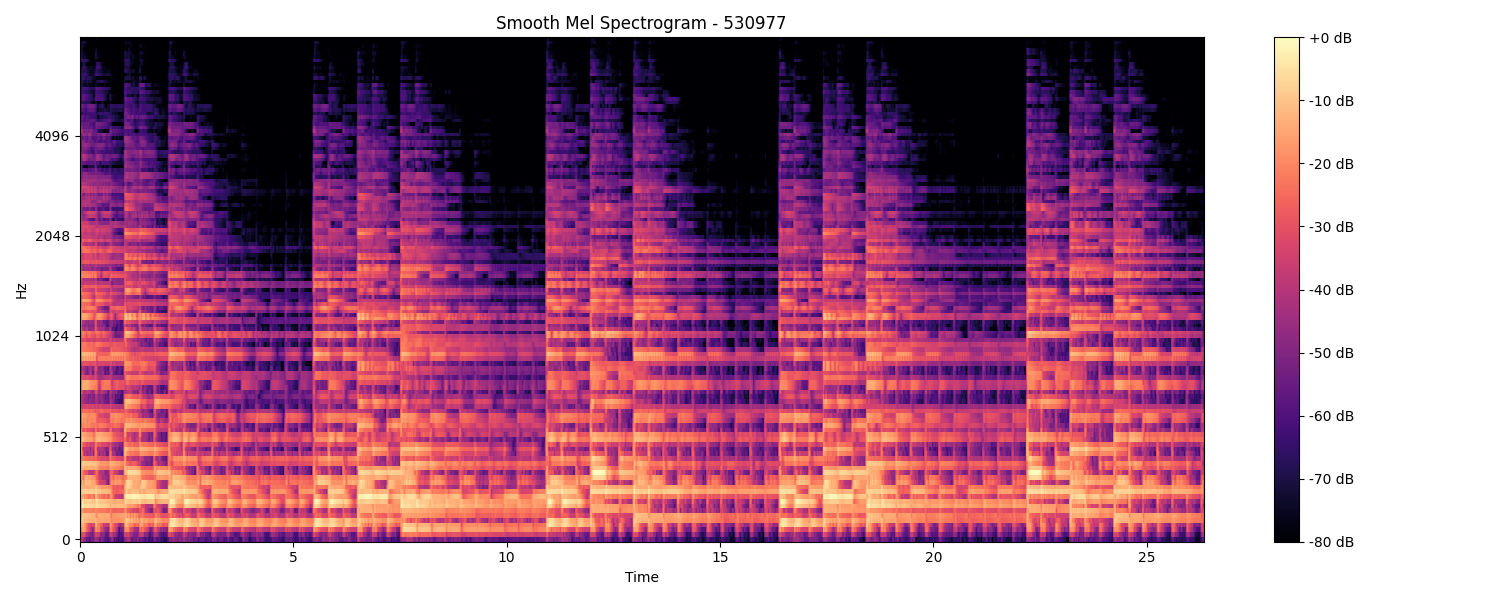
\includegraphics[width=\textwidth]{figures/530977_plot.png}
        \label{fig:task7_1}
    \end{subfigure}
    \hfill
    \begin{subfigure}[b]{0.48\textwidth}
        \centering
        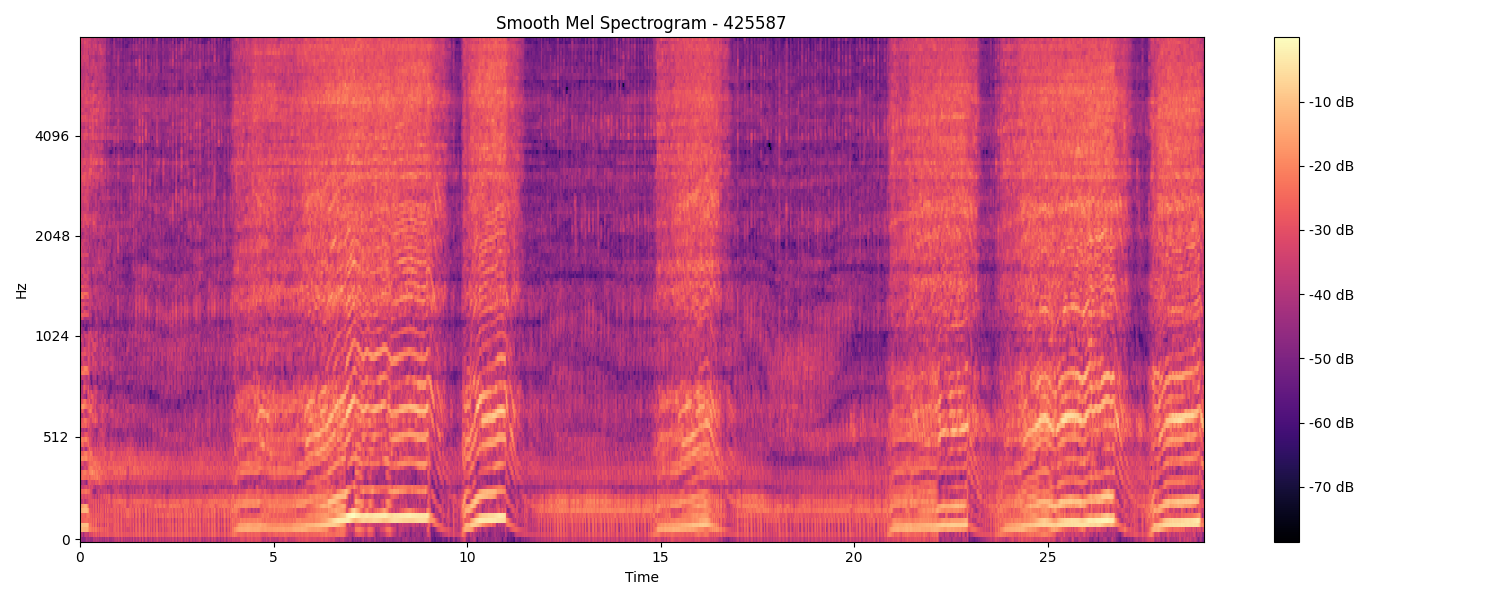
\includegraphics[width=\textwidth]{figures/425587_plot.png}
        \label{fig:task7_1_2}
    \end{subfigure}
    \hfill
    \caption{Smooth mel spectrograms of two unseen test audio files.}
    \label{fig:Task7_A}
\end{figure}

\begin{table}[ht]
\centering
\begin{minipage}{0.48\textwidth}
\centering
\caption{Audio 530977: Classes and Frame Counts}
\begin{tabular}{l r}
\hline
\textbf{Class Name} & \textbf{Sum over Time (Frames)} \\
\hline
Guitar & 129 \\
Piano  & 219 \\
\hline
\end{tabular}
\end{minipage}%
\hfill
\begin{minipage}{0.48\textwidth}
\centering
\caption{Audio 425587: Classes and Frame Counts}
\begin{tabular}{l r}
\hline
\textbf{Class Name} & \textbf{Sum over Time (Frames)} \\
\hline
Chainsaw & 243 \\
\hline
\end{tabular}
\end{minipage}
\end{table}

\subsection{Auditory Inspection of Classifier Predictions}
Listening to the audio files (played in the notebook) allows a subjective assessment:
\begin{itemize}
    \item For 530977, the sounds of guitar and piano are perceptible and the classifier accurately detects their presence during the corresponding time frames, showing it can recognize prominent musical instruments effectively.
    \item For 425587, the chainsaw sound is dominant and the model’s prediction strongly reflects this. This suggests the model performs well on prominent, distinctive environmental sounds.
\end{itemize}

The qualitative inspection confirms the classifier’s predictions match audible events quite well for clear and distinctive classes.

\subsection{Problematic Conditions and Postprocessing Suggestions}
Potential problematic conditions causing mispredictions or missed detections include:
\begin{itemize}
    \item Overlapping sounds or noisy environments where multiple sources mix, confusing the model.
    \item Subtle or low-volume events that might be below the detection threshold.
    \item Short, transient sounds that may be temporally smoothed out or missed in frame-level predictions.
\end{itemize}
Simple postprocessing steps that might help:
\begin{itemize}
    \item Temporal smoothing (median filtering): Reduces noisy frame-level fluctuations.
    \item Threshold tuning: Adjusting detection thresholds per class could help balance false positives/negatives.
    \item Context-aware smoothing: Using longer temporal context or a postprocessing HMM/CRF to enforce temporal consistency.
    \item Ensemble models: Combining multiple models trained with different features or architectures for robust predictions.  
\end{itemize}



\end{document}